\chapter{Theoretischer Teil}
\label{chapter_TheoretischerTeil}
Dieses Kapitel befasst sich mit den theoretischen Grundlagen, die für den Einsatz von \acp{SBC} zur Datenerfassung mittels verschiedenen Sensoren nötig sind. In Abschnitt \ref{section_Begriffsdefiniton} werden die im weiteren Verlauf der Arbeit verwendeten Fachbegriffe erläutert, um die beschriebenen Zusammenhänge gut zu verstehen. Der Abschnitt \ref{section_Vergleich_SBC} behandelt die unterschiedlichen sich auf dem Markt befindenden \acp{SBC} mit ihren jeweiligen Vor- bzw. Nachteilen. Die verschiedenen Bussysteme wie z.B. der \ac{I$^2$C}  Bus werden in Abschnitt \ref{section_Bussysteme} erklärt und deren Funktionsweise erläutert. 


\section{Begriffsdefinition}
\label{section_Begriffsdefiniton}
Die in diesem Abschnitt beschriebenen Definitionen wurden, soweit nicht anders angegeben aus folgendem Dokument entnommen \citep{Bussysteme_in_der_Praxis}.

\subsection*{Single Board Computer}
Unter einem \textit{Single Board Computer} (\ac{SBC}) versteht man ein Computersystem, welches sich komplett auf einer einzigen Platine befindet. \acp{SBC} können fast die gleichen Aufgaben erledigen wie gewöhnliche Computer, allerdings sind die Einplatinen Rechner diesen in Hinblick auf die Hardwareausstattung doch um einiges unterlegen.

\subsection*{Bussysteme}
\textit{Bussysteme} sind Systeme, die verwendet werden zur seriellen Datenübertragung zwischen einen oder mehreren Komponenten. Beispiele hierfür sind der \ac{I$^2$C} Bus, der \ac{SPI} Bus oder auch der \ac{CAN} Bus. Eine genauere Beschreibung der einzelnen Bussysteme folgt in Abschnitt \ref{section_Bussysteme}.

\subsection*{Raspberry Pi}
Der \textit{\ac{RPI}} ist ein \ac{SBC}, der von der britischen \textit{Raspberry Pi Foundation} aus Komponenten von Android-Smartphones entwickelt wurde.

\subsection*{Raspbian}
\textit{Raspbian} ist ein Betriebssystem, welches auf der Linux Distribution Debian basiert und speziell auf den Raspberry Pi angepasst wurde.

\subsection*{RRDTool}
Das \textit{RRDTool} ist ein Programm, mit dem man Round-Robin Datenbanken erstellen kann. Diese Datenbanken eignen sich besonders gut für die Aufzeichnung von zeitlich fortlaufenden Datenreihen wie z.B. Temperaturmessungen oder Strommessungen. Die Datenbank liegt dabei in einem einzigen File auf dem Datenträger und hat ab dem Erstellen eine feste Größe, die sich auch bei vielen Messungen über einen längeren Zeitraum nicht vergrößert. 

\subsection*{General Purpose Input/Output}
Unter \textit{\ac{GPIO}} versteht man elektrische Kontakte, die zur Realisierung verschiedener Funktionen für elektronische Geräte verwendet werden. Eine genauere Erklärung erfolgt in Abschnitt \ref{subsection_GPIO} \citep{Raspberri_Pi_Handbuch}.
\subsection*{Python}
\textit{Python} ist eine Programmiersprache, die vor allem auf dem Raspberry Pi bevorzugt verwendet wird.
\subsection*{Bluetooth Low Energy}
\textit{\ac{BLE}} ist eine Funktechnologie, die es ermöglicht, dass sich Geräte in unmittelbarer Entfernung zueinander vernetzen lassen. Die Stromkosten bei \ac{BLE} sind um einiges geringe als bei herkömmlichen Bluetooth \citep{Bluetooth_Low_Energy}.
\subsection*{Windows 10 IoT}
\textit{Windows 10 IoT} ist eine \glqq abgespeckte\grqq Version von Windows 10, die auf Mobilen Geräten wie dem Raspberry Pi lauffähig ist. IoT steht dabei für \textit{Internet of Things} \citep{Raspberri_Pi_Handbuch}.

%Abschnitt Vergleich von SBCs 
\section{Vergleich von verschiedenen SBC}
\label{section_Vergleich_SBC}
In diesem Abschnitt werden einige der bekanntesten \acp{SBC}, die sich auf dem Markt befinden miteinander verglichen, um den bestmöglichen für die vorgegebenen Anforderungen auswählen zu können.
Wichtige Kriterien für die Auswahl sind, dass die Möglichkeit besteht verschiedene Betriebssysteme (Windows und Linux) mit dem jeweiligen Einplatinenrechner betreiben zu können, sowie die verbaute Hardware(Taktfrequenz des Chips, RAM-Speicher). Ein weiterer Punkt welcher von Bedeutung ist, ist die Unterstützung von verschiedenen Kommunikationsschnittstellen (\ac{I$^2$C}, \ac{SPI}, 1-Wire), um eine große Anzahl von Sensoren nutzen zu können. Eine Übersicht der einzelnen Komponenten der verschiedenen \acp{SBC} sind in den Tabellen \ref{Tabelle_Vergleich_SBC1} und \ref{Tabelle_Vergleich_SBC2} dargestellt.

%Tabelle 1
\begin{table}[H]
%\rowcolors{2}{black!10}{black!20}
\centering
\begin{tabular}{
llll
}
\toprule
\multicolumn{1}{p{3cm}}{\textit{\ac{SBC}}} & \multicolumn{1}{p{3.5cm}}{\textit{Operating System} } & \multicolumn{1}{p{1,5cm}}{\textit{RAM} }&\multicolumn{1}{p{3cm}}{ \centering\textit{CPU} }\\\midrule
Banana Pi & Linux, Android & 1 GB & ARM Cortex-A7, 1 GHz\\
&&&\\
Raspberry Pi2&Windows, Linux&1 GB&ARM Cortex-A7 900 MHz\\
&&&\\
Raspberry Pi3&Windows, Linux&1 GB&ARM Cortex-A53 1,2 GHz\\
&&&\\
BeagleBone Black & Linux & 512 MB & ARM Cortex-A8 1 GHz\\
&&&\\
HummingBoard i2eX & Linux, Android & 1 GB & ARM Cortex-A9 1 GHz\\
&&&\\
Intel Galileo Gen 2 & Windows, Linux & 256 MB & x86 Quark 400 MHz\\
&&&\\
Radxa Rock & Linux & 2 GB & ARM Cortex-A9 1,6 GHz\\
\bottomrule
\end{tabular}
\caption{Vergleich OS, RAM, CPU verschiedener SBCs}
\label{Tabelle_Vergleich_SBC1}
\end{table}

\begin{threeparttable}[H]
%\rowcolors{2}{black!10}{black!20}
\centering
\begin{tabular}{
llll
}
\toprule
\multicolumn{1}{p{3cm}}{\textit{\ac{SBC}}} & \multicolumn{1}{p{3.5cm}}{\textit{Communication} } & \multicolumn{1}{p{3cm}}{\textit{Networking} }&\multicolumn{1}{p{3cm}}{ \textit{GPIO} }\\\midrule
Banana Pi & I$^2$C, SPI & 1\;GigE & 80\\
&&&\\
Raspberry Pi2&I$^2$C, SPI&10/100\;Mbps&40\\
&&&\\
Raspberry Pi3&I$^2$C, SPI&10/100\;Mbps\tnote{1} &40\\
&&&\\
BeagleBone Black &I$^2$C, SPI&10/100\;Mbps&66\\
&&&\\
HummingBoard i2eX &I$^2$C, SPI&1\;GigE&8\\
&&&\\
Intel Galileo Gen 2 & I$^2$C, SPI&10/100\;Mbps&20\\
&&&\\
Radxa Rock & I$^2$C, SPI\tnote{2}&10/100\;Mbps&80\\
\bottomrule
\end{tabular}

\begin{tablenotes}\footnotesize
\item[1] mit WLAN on Board
\item[2] nur für Android
\end{tablenotes}

\caption{Vergleich Schnittstellen, Netzwerkverbindung, Anzahl GPIO Pins}
\label{Tabelle_Vergleich_SBC2}
\end{threeparttable}

Wie aus den Tabellen ersichtlich ist, unterstützen die meisten aktuellen \acp{SBC} das Betriebssystem Linux. Eine Anforderung für diese Projekt war allerdings, dass sowohl ein Linux System, wie auch ein Windows System auf dem Board lauffähig ist. Aus diesem Grund fiel die Wahl auf den \ac{RPI}\;3, da dieser beide Betriebssysteme unterstützt und auch bei den anderen betrachteten Aspekten wie \textit{RAM, CPU} etc. den meisten Boards ebenbürtig oder sogar überlegen ist. Ein weiterer wichtiger Entscheidungsgrund für den \ac{RPI}\;3 war, dass es für diesen eine sehr große Anzahl an unterstützten Sensoren gibt (Sensoren die mit einer elektrischen Spannung von 3,3\;$V$ - 5\;$V$) betrieben werden. Dies ermöglicht einen sehr weit gefächerten Einsatz des \ac{RPI}\;3 und ist für das vorgesehene Projekt von großer Bedeutung.

%%Kapitel Raspberry PI
\section{Raspberry Pi 3}
\label{section_Raspberry_Pi3}
Das folgende Kapitel beschreibt den Raspberry Pi 3 und befasst sich genauer mit den verbauten Komponenten, welche im weiteren Verlauf der Arbeit benötigt werden. 

\subsection{Allgemeine technische Daten}
\label{subsection_Allgemeine_technische_Daten}
Die im folgenden Information wurden, soweit nicht anders angegeben von der offiziellen Homepage der \textbf{Raspberry Pi Foundation} entnommen \citep{RaspberryPiHomePage}.\\
Der \ac{RPI} 3 ist ein Kreditkarten großer Einplatinenrechner, welcher aktuell an die \textit{sieben Million} Mal verkauft wurde \citep{RPI_Verkaufszahlen}. Dieser besitzt\dots
\begin{itemize}
\item einen 1.2\;GHz 64-bit quad-core ARMv8 CPU
\item 802.11n Wireless LAN
\item Bluetooth 4.1
\item \ac{BLE}
\item 4 USB Ports
\item 40 GPIO Pins
\item Full HDMI Port
\item Ethernet Port
\item \ac{CSI}
\item \ac{DSI}
\item Micro SD Karten Slot
\end{itemize}

Die aktuelle Version des Raspberry Pi, der \ac{RPI}\;3 ist in Abbildung \ref{Abb_Bild_RPI3} dargestellt.

\begin{figure}[!h] 
  \centering
     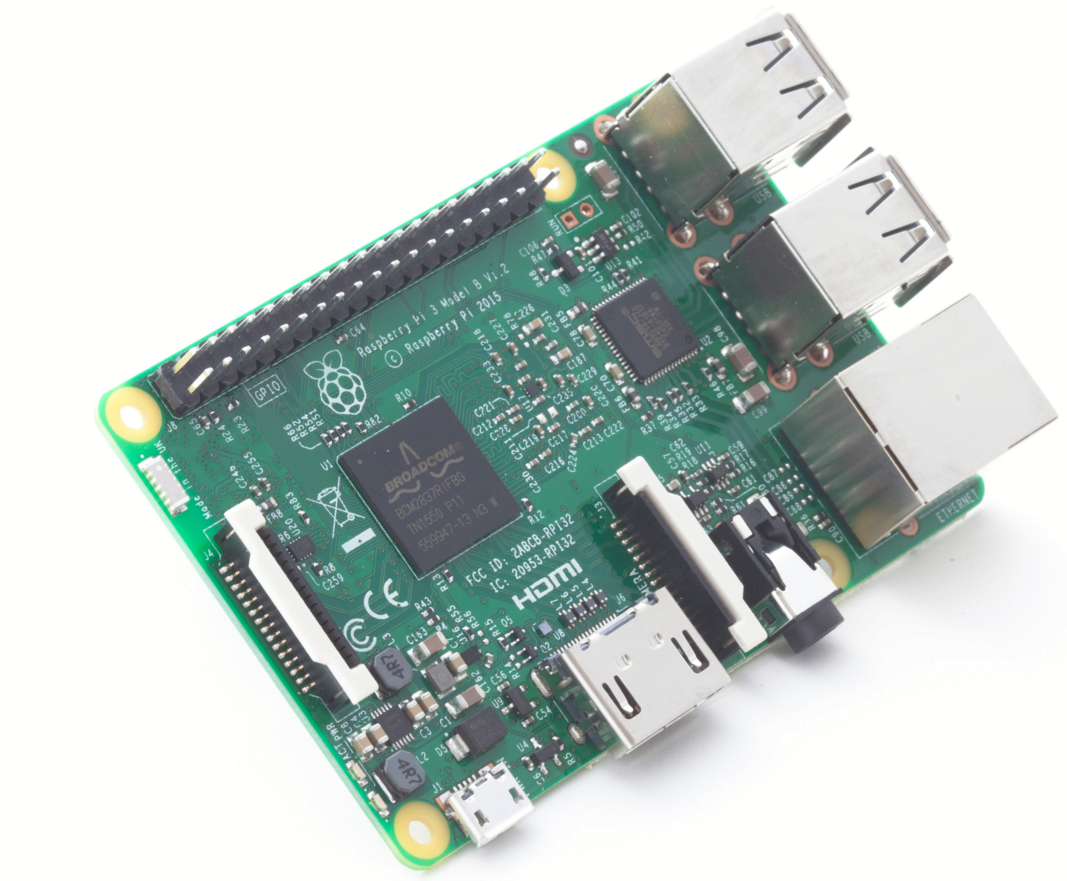
\includegraphics[scale=.4]{BilderAllgemein/RPI3.png}
  \caption{Raspberry Pi\;3 \citep{RPI_Bild}}
  \label{Abb_Bild_RPI3}
\end{figure}

Durch die im Gegensatz zu den Vorgänger Modellen leistungsstärkere CPU mit einem 64-Bit quad-core Prozessor, ist es beim RPI\;3 möglich das Windows Betriebssystem \textit{Windows 10 IoT} auf dem Gerät zu betreiben, wodurch sich eine Erweiterung der Einsatzmöglichkeiten (nicht mehr nur auf Linux Betriebssysteme beschränkt) ergibt. Auch wurde im Gegensatz zu den vorherigen Modellen beim aktuellen ein WLAN Modul (2,4\;GHz) gleich auf der Platine verbaut und muss nicht mehr extra durch ein externes USB-WLAN Modul realisiert werden. Der \ac{RPI}3 bietet weiterhin einen 10/100 MBit Ethernet Anschluss sowie einen \ac{CSI} und \ac{DSI} Anschluss zur direkten Anbindung einer Kamera oder Displays. Die verschiedenen GPIO-Pins werden in Kapitel \ref{subsection_GPIO} genauer beschrieben.

\subsection{GPIO-Kontakte}
\label{subsection_GPIO}
Wie bereits in Abschnitt \ref{subsection_Allgemeine_technische_Daten} angesprochen besitzt der \ac{RPI}\,3 40 GPIO-Kontakte, welche in einer Ecke der Platine zu 2\;x\;20 Kontakten angeordnet sind. Diese haben einen Rasterabstand von 2,54 mm zueinander und stellen die Grundlage für viele Projekte dar. Die ersten Modelle des \ac{RPI} besaßen dagegen nur 26 Pins die zur Verfügung standen. Die GPIO-Pins sind elektrische Kontakte, die zur Messung und Steuerung von elektronischen Geräten wie z.B. Sensoren, Analog Digital Wandlern, LEDs etc. verwendet werden.\\
Die Steckerleiste beinhaltet einige allgemein verwendbare Pins (\textit{=\;General Purpose Input\;/\;Output}), sowie zwei verschiedene Spannungsversorgungen (\textit{3,3\;V} und \textit{5\;V}) und Masse Anschlüsse (\textit{0\;V}). Weiterhin beinhaltet die Steckerleiste Kontakte für den \ac{I$^2$C}-, \ac{SPI}- und 1-Wire-Bus. Bei der Verwendung der GPIO-Kontakten für verschiedene Projekte, muss darauf geachtet werden, welche Bezeichnung verwendet wird. Diese ist in vielen Literaturen verschieden angegeben, da es drei verschiedene Möglichkeiten der Bezeichnung gibt. Die Benennung kann durch
\begin{itemize}
\item die physikalische Pin-Nummer, anhand seine Position auf dem Board (von oben gesehen, Pin 1 besitzt eine quadratische Lötstelle)
\item die BCM-Pin-Nummer, welche sich auf die Nummerierung der offiziellen Dokumentation des BCM2836-Chips bezieht
\item den Pin Namen, welcher von den \ac{RPI} Entwicklern vergeben wurde 
\end{itemize} 
vorgenommen werden \citep{Raspberri_Pi_Handbuch}.\\\\
In Abbildung ist die Pin Belegung des \ac{RPI} grafisch dargestellt.

%Grafik GPIO Pins
\begin{figure}[!h] 
  \centering
     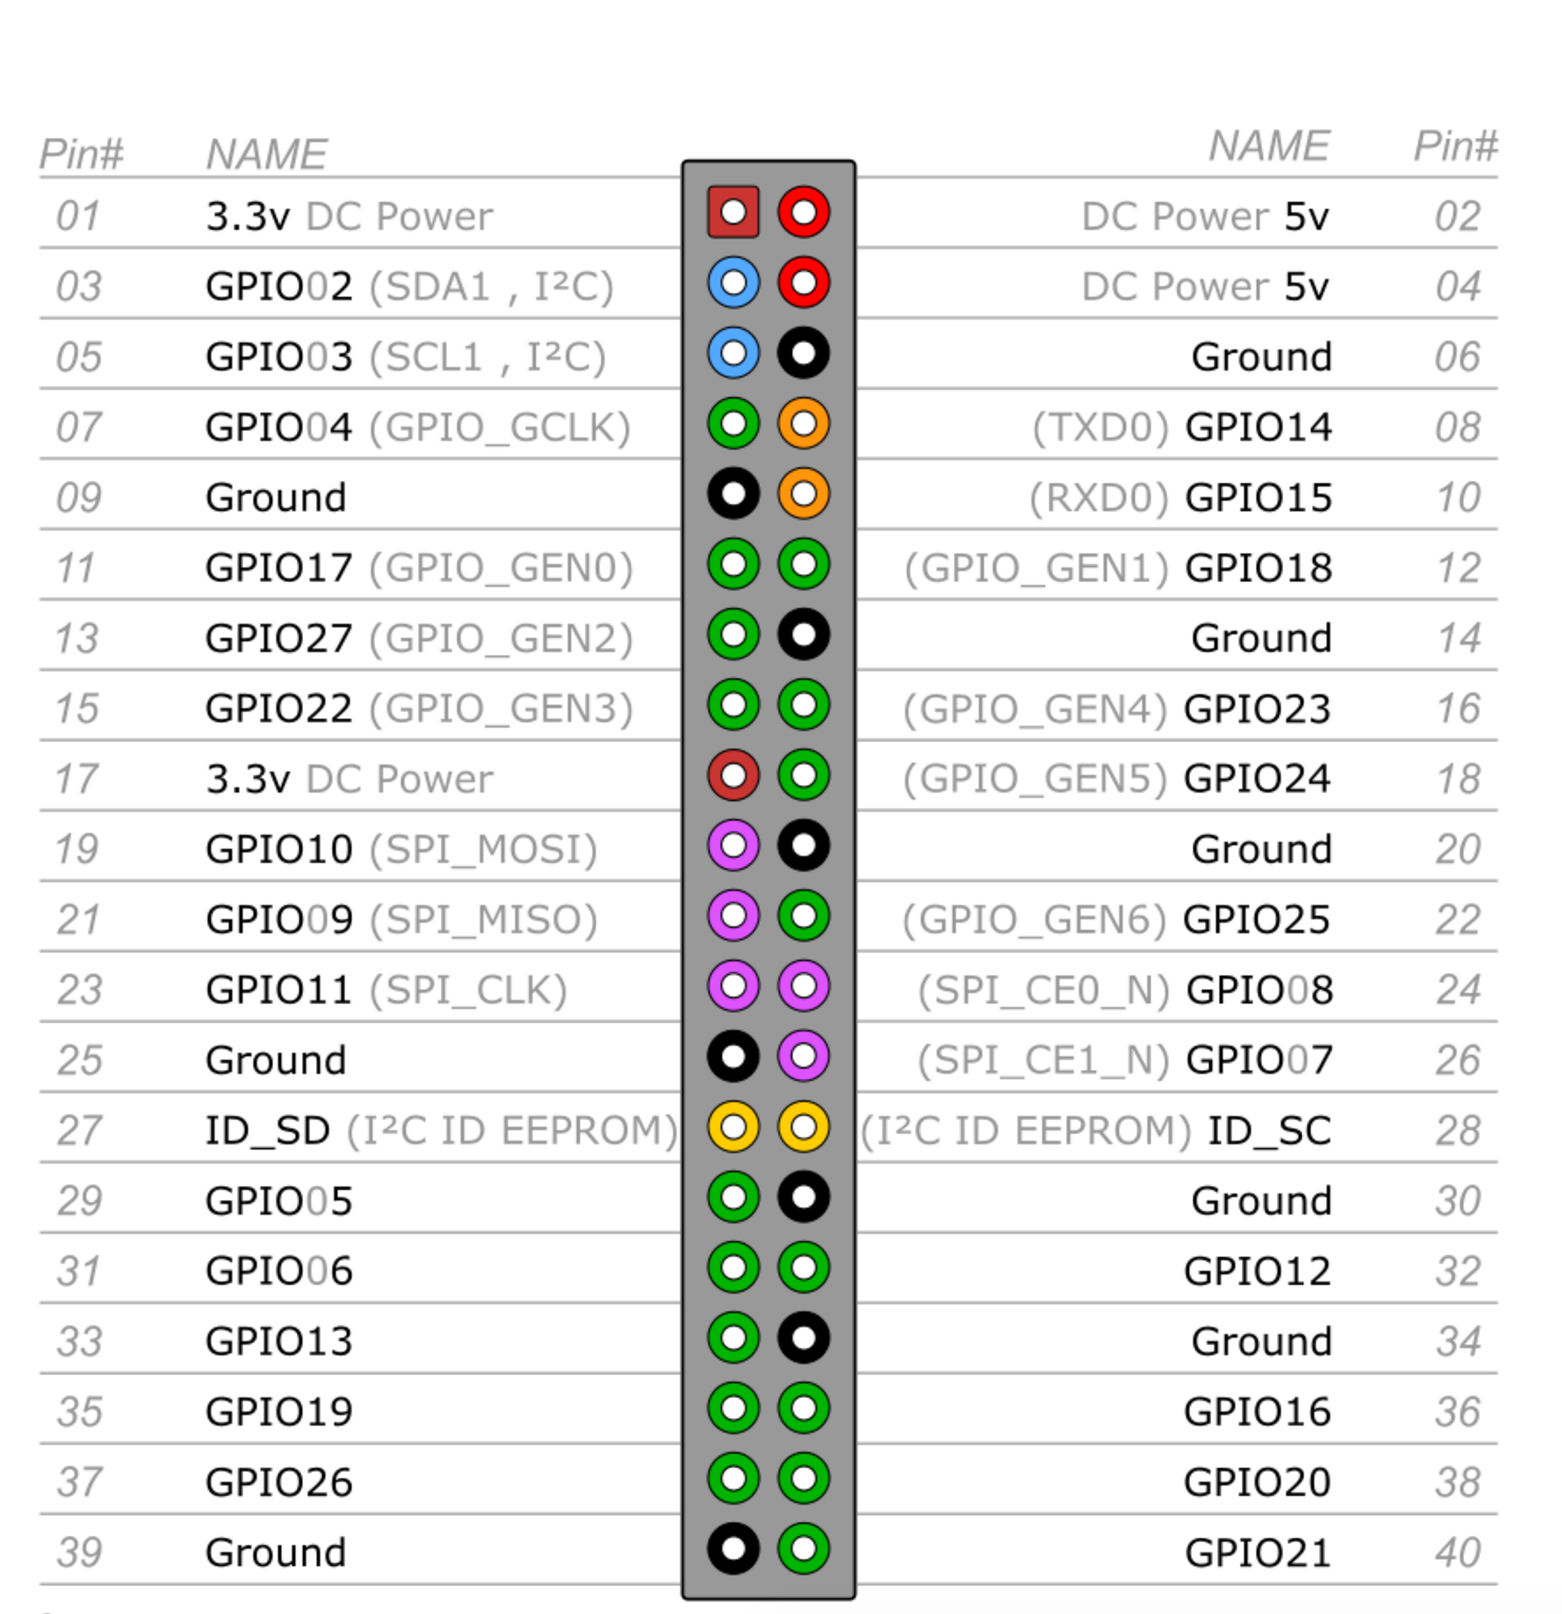
\includegraphics[scale=.35]{BilderAllgemein/GPIO.png}
  \caption{GPIO-Header \citep{GPIO_Header_Bild}}
  \label{Abb_Bild_GPIO}
\end{figure}

%% Section Bussysteme
\section{Bussysteme}
\label{section_Bussysteme}
Im folgenden Kapitel werden die am häufigsten verwendeten Bussysteme für die verschiedenen Sensoren erläutert. Zu diesen Bussystemen gehören der \textit{1-Wire}, \textit{\ac{I$^2$C}} und der \textit{\ac{SPI}} Bus. Auch wird auf die Funktion, sowie die Eigenheiten der Datenübertragung des jeweiligen Busses eingegangen.

\subsection{1-Wire}
\label{subsection_1Wire}
Der 1-Wire Bus ist ein serielles Bussystem von der Firma \textit{Dallas\footnote{2001 von Maxim Integrated übernommen}} , bei dem die Daten seriell (nacheinander) über eine Datenleitung übertragen werden.
\subsubsection{Allgemeine Informationen}
\label{subsection_Allgemeine_Informationen_1Wire}
 Für dieses Bussystem wird nur eine Datenleitung benötigt, die auch als Spannungsversorgung für den\;/\;die jeweiligen Sensoren benutzt wird. Physikalisch werden allerdings zwei Leitungen benötigt, da die Masse auch mitgeführt werden muss. Es gibt für diesen Bus eine große Anzahl an Sensoren wie z.B. Temperatursensoren, die sich durch einen sehr geringen Stromverbrauch auszeichnen. Dies kommt daher, da für die Datenübertragung und die Stromversorgung die gleiche Leitung genutzt wird, wird während der Kommunikation der Sensor aus einem internen Kondensator gespeist. Allerdings kann es notwendig sein, bei Sensoren wo die interne Spannungsversorgung nicht ausreichend ist  eine extra Spannungsversorgung für den jeweiligen Sensor mitzuführen. \\
Diese System ist ein \textit{One-Master-Multi-Slave} Bussystem, was bedeutet, dass es nur einen Master (z.B. \ac{RPI}) gibt aber mehrere Slaves (z.B. Sensoren). Die Aufgabe des Masters in diesem System ist es, die Kommunikation zu steuern. Die Anzahl der Sensoren kann bis zu 100 betragen, die parallel an den Master angeschlossen werden. Dies ist möglich, da jeder Sensor ein eindeutige 64 Bit lange ID besitzt. Diese gliedert sich in \citep{Bussysteme_in_der_Praxis}
\begin{itemize}
\item 8 Bit \textit{Family Code}
\item 48 Bit \textit{Seriennummer}
\item 8 Bit \textit{CRC-Prüfsumme}
\end{itemize}

\subsubsection{Übertragungsprotokoll}
\label{subsection_Protokoll_1Wire}
Der 1-Wire Bus wird dadurch, dass er keine Taktsignal benötigt als \textit{asynchroner} Bus bezeichnet. Dieser kommuniziert im \textit{Halbduplex} Verfahren, was bedeutet, dass immer nur ein Teilnehmer auf dem Bus senden oder empfangen kann (entweder Master oder ein Slave). Wenn keine Kommunikation stattfindet, wird die Datenleitung über einen Pullup-Widerstand auf \textit{high} gezogen und der in Abschnitt \ref{subsection_Allgemeine_Informationen_1Wire} erwähnte interne Kondensator geladen. In dem andern Fall wenn eine Übertragung stattfindet liegt die Datenleitung auf Masse und der Kondensator liefert in diesem Fall die Spannungsversorgung für den Sensor (abhängig vom Sensor siehe \ref{subsection_Allgemeine_Informationen_1Wire}). Da wie schon angesprochen keine Taktleitung vorhanden ist, muss für die Kommunikation ein bestimmter Ablauf eingehalten werden. Dafür gibt es zwei Übertragungsmöglichkeiten, den \textit{normalen Modus} wo ca. 16,3\;$kBit/s$ übertragen werden und den \textit{Overdrive Modus} mit bis zu 142\;$kBit/s$.\\
Die Zeitspanne für die Übertragung von 1 Bit beträgt immer 60\,$\mu s$. Diese Steuerung, egal in welche Richtung die Übertragung stattfindet werden durch den Master initiiert. Die Befehle die dazu notwendig sind, können aus der Tabelle \ref{Tabelle_Befehle_1Wire} entnommen werden \citep{Bussysteme_in_der_Praxis}.

%Tabelle 1
\begin{table}[H]
%\rowcolors{2}{black!10}{black!20}
\centering
\begin{tabular}{
llll
}
\toprule
\multicolumn{1}{p{2cm}}{\textit{Befehl} }&\multicolumn{1}{p{10cm}}{\centering\textit{Beschreibung} }\\\midrule
\textbf{Write 1} & Der Master zieht für $1-15\;\mu s$ auf Low. Der Rest des Slots bleibt \\
& ungenutzt.\\
&\\
\textbf{Write 0} & Der Master zieht den Bus für mindestens $60\;\mu s$ bis maximal\\
& $120\;\mu s$ auf Low.\\
&\\
\textbf{Read}& Der Master zieht für $1-15\;\mu s$ auf Low. Der Slave, der kommunizieren\\
& möchte, hält für eine 0 den Bus weiter auf Low. Will der Slave eine\\
& 1 senden, gibt er direkt den Bus wieder frei. Wie man leicht erkennt,\\
& ist der Status \textit{Write 1} oder Read für den Master gleich.\\
& Alleine der Status des Sensors bestimmt, ob ein Read oder Write 1 \\
& ausgeführt wird.\\
&\\
\textbf{Reset /} & Der Master zieht den Bus für min. $480\;\mu s$ auf Low. Wenn ein\\
\textbf{Presence} & Slave am Bus vorhanden ist, zieht er max. $60\;\mu s$ (also einen\\
& Slot) die Leitung auf Low. Somit weiß der Master, dass mindestens\\
& ein Slave angeschlossen ist.\\ 
\bottomrule
\end{tabular}
\caption{Befehle bei 1-Wire \citep[S. 35]{Bussysteme_in_der_Praxis}}
\label{Tabelle_Befehle_1Wire}
\end{table}

%I2C Bus
\subsection{I$^2$C-Bus}
\label{subsection_I2C}
Der \ac{I$^2$C} Bus ist auch noch unter einem anderen Namen als \ac{TWI} Bus (z.B. bei Atmel) bekannt. Er wurde 1982 von der Firma Philips Semiconductors\footnote{heute NPX} entwickelt und wird vornehmlich zur internen Kommunikation von Geräten benutzt \citep{Bussysteme_in_der_Praxis}.

\subsubsection{Allgemeine Informationen}
\label{subsubsection_Allgemeine_Informationen_I2C}
Technisch gesehen sind der \ac{I$^2$C} und \ac{TWI} Bus identisch, die Unterscheidung wird lediglich aus Lizenz rechtlichen Gründen getroffen. Bei dem Bus handelt es sich um einen \textit{Master-Slave-Bus}, allerdings ist auch ein \textit{Multi-Master\footnote{es gibt mehr als einen Master}} Betrieb möglich. Der Beginn einer Kommunikation wird immer vom Master initiiert, bei dem angesprochenen Multi-Master Betrieb, arbeitet dann der vom Initiator angesprochene Master wie ein Slave. Im Gegensatz zum 1-Wire Bus sind zwei Leitungen notwendig, eine Datenleitung (SDA) und eine Taktleitung (SCL). Da der \ac{I$^2$C} Bus eine Taktleitung besitzt, spricht man hier von einem synchronen seriellen Bussystem. Der Systemtakt wird bei diesem System immer vom Master vorgegeben. 

\subsubsection{Ad}
\subsubsection{Übertragungsprotokoll}
\label{subsubsection_Übertragungsprotokoll_I2C}
Für eine fehlerfreie Übertragung bei dem \ac{I$^2$C} Bussystem müssen bestimmte Bedingungen eingehalten werden.\\
Damit ein Bit auf der Datenleitung als gültig betrachtet wird, darf sich dessen Pegel während der High Phase der Taktleitung nicht ändern (siehe Abbildung \ref{Abb_Bild_I2C_data_valid})

%Grafik Data valid
\begin{figure}[!h] 
  \centering
     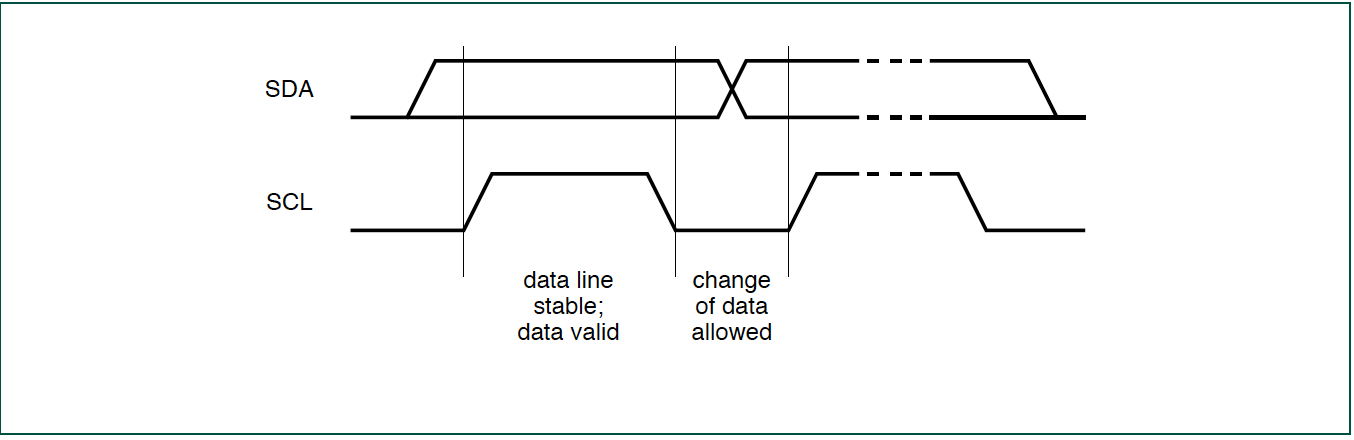
\includegraphics[scale=.65]{BilderAllgemein/I2C_data_valid.png}
  \caption{Bedingung für gültiges Bit auf Datenleitung \citep[S. 8]{I2C_Datenblatt}}
  \label{Abb_Bild_I2C_data_valid}
\end{figure}


\subsection{SPI-Bus}
\label{subsection_SPI}
